\documentclass[a4paper,10pt]{article}
\usepackage[utf8x]{inputenc}
\usepackage[T1]{fontenc}
\usepackage[french]{babel}

\usepackage{algorithmic}
\usepackage{algorithm}
\usepackage{graphicx}
\usepackage{multirow}

\usepackage{common-formatting}
\usepackage{common-math}

%opening
\title{TP3 - Projets déterministes - MACS1}
\author{Alexandru Fikl}

\begin{document}

\maketitle

\section{Méthodes de Newton-Coates}
Les méthodes de Newton-Cotes sont les méthodes d'intégration numérique du type:
\[
\int_a^b f(x) \dx{x} = \sum_{i = 1}^n \omega_i f(x_i).
\]

\begin{enumerate}
    \item \emph{Expliciter les formules d'intégration numérique de la méthode des
    rectangles (autrement appelée méthode des escaliers), du point milieu, du
    trapèze, de Simpson $\frac{1}{3}$ et $\frac{1}{8}$.}

    Soient une fonction $f$ suffisament régulière sur l'interval $[a, b]$ et
    $(x_i)_{i \in \llbracket 0, n \rrbracket}$ la discrétisation régulière de
    l'interval $[a, b]$ définie par:
\[
    \forall i \in \llbracket 0, n \rrbracket,~ x_i = a + ih \text{ avec }
    h = \frac{b - a}{n}.
\]

    Alors les formules sont:
    \begin{description}
        \item[Rectangle:] $\displaystyle \int_a^b f(x) \dx{x} \approx h
        \sum_{i = 1}^{n - 1} f(x_{i + 1})$
        \item[Point Milieu:] $\displaystyle \int_a^b f(x) \dx{x} \approx h
        \sum_{i = 1}^{n - 1} f(\frac{x_i + x_{i + 1}}{2})$
        \item[Trapèze:] $\displaystyle \int_a^b f(x) \dx{x} \approx \frac{h}{2}
        \sum_{i = 1}^{n - 1} (f(x_i) + f(x_{i + 1}))$
        \item[Simpson $\frac{1}{3}$:] $\displaystyle \int_a^b f(x) \dx{x} \approx
        \frac{h}{6}\sum_{i = 1}^{n - 1} (f(x_i) + 4f(\frac{x_i + x_{i + 1}}{2}) +
        f(x_{i + 1}))$
        \item[Simpson $\frac{1}{8}$:] $\displaystyle \int_a^b f(x) \dx{x} \approx
        \frac{h}{8}\sum_{i = 1}^{n - 1} (f(x_i) + 3f(\frac{2x_i + x_{i + 1}}{3}) +
        3f(\frac{x_i + 2x_{i + 1}}{3}) + f(x_{i + 1}))$
    \end{description}

    \item \emph{Implémenter ces méthodes en matlab. (chaque fonction d'intégration
    numérique devra prendre en arguments d'entrée l'intervalle sur lequel on intégre,
    le nombre de discrétisation de l'intervalle et la fonction que l'on souhaite
    intégrer et en argument de sortie la valeur de l'intégrale). Ne pas oublier les
    commentaires.}

    Voir les fichiers $Rectangle.m$, $MiddlePoint.m$, $Trapezoid.m$,
    $Simpson13.m$ et $Simpson38.m$ pur le code MATLAB.

    \item \emph{Tester ces méthodes sur des exemples de votre choix. On créera au moins
    autant de script de test que de méthodes à tester (plus si affinités).}

    Voir le fichier \emph{ex1\_test\_newton\_coates.m}.

    \item \emph{Tracer les courbes d'erreur pour chacune des méthodes en log-log (on
    pourra tracer sur les mêmes graphes des droites de différents ordres pour
    identifier les ordres). Il faut donc tracer la norme de l'erreur en fonction
    du nombre de discrétisations de l'interval (il faudra donc lancer le calcul de
    l'intégrale avec des discrétisations de plus en plus fines : typiquement on
    double les discrétisations à chaque fois, donc on divise par deux le pas de
    discrétisation). Vérifier que les ordres obtenus correspondent aux ordres
    théoriques et vérifier sur des exemples appropriés l'exactitude de méthodes
    (ex : une méthode d'ordre 1 est exacte lorsque l'on intégre exactement des
    polynômes d'ordre 0).}

    L'ordre de chaque méthode est:
    \begin{description}
        \item[Rectangle] a ordre 1,
        \item[Point Milieu] a ordre 2,
        \item[Trapèze] a ordre 2,
        \item[Simpson $\frac{1}{3}$] a ordre 4 et
        \item[Simpson $\frac{1}{8}$] a aussi ordre 4.
    \end{description}

    Nous pouvons bien voir ça dans la Figure~\ref{fig:order}.

    Pour tester l'ordre de chaque méthode, nous prenons la valeur de l'intégrale des
    fonctions suivantes sur l'interval $[0, 1]$ avec $200$ discrétisations:

{
\renewcommand{\arraystretch}{1.2}
\begin{center}
\begin{tabular}{|l|l|l|l|l|l|l|}\hline

\multirow{2}{*}{Fonction} & \multirow{2}{*}{Solution} & \multicolumn{5}{c|}{Erreur} \\\cline{3-7}
      &         & Rectangle & Point Milieu & Trapèze & Simpson $\frac{1}{3}$ & Simpson $\frac{1}{8}$\\\hline
$x^0$ & 1       & 0         & 0            & 0       & 0                    & 0 \\\hline
$x^1$ & 0.5     & 0.025     & 0            & 0       & 0                    & 0 \\\hline
$x^2$ & 0.333   & 0.024     & 2e-6         & 4.1e-6  & 0                    & 0 \\\hline
$x^3$ & 0.25    & 0.024     & 3.1e-6       & 6.2e-6  & 0                    & 0 \\\hline
$x^4$ & 0.2     & 0.024     & 4.1e-6       & 8.3e-6  & 5.2e-12              & 2.3e-12 \\\hline
$x^5$ & 0.166   & 0.024     & 5.2e-6       & 1.05e-6 & 1.3e-11              & 5.7e-12 \\\hline

\end{tabular}
\end{center}
}
\end{enumerate}

\section{Calculs d'intégrales généralisées}

On va appliquer les méthodes précédentes de calcul d'intégrales sur différents
exemples:

\begin{enumerate}
    \item \emph{Tester vos codes sur des fonctions fortement oscillantes (par rapport à
    l'intervalle de discrétisation); puis commenter les résultats.}

    Soit la fonction $f(x) = 7\cos(23x)$ sur l'interval $[0, \frac{5 \pi}{2}]$
    en fixant le nombre de discrétisations. (voir Figure~\ref{fig:osc})

{
\renewcommand{\arraystretch}{1.2}
\begin{center}
\begin{tabular}{|l|l|l|l|l|l|l|}\hline

Iterations & Solution & Rectangle & Point Milieu & Trapèze & Simpson $\frac{1}{3}$ & Simpson $\frac{1}{8}$\\\hline
10         & -0.3043  & 3.8875    & -7.1832      & 6.6364  & -2.5766              & 7.0 \\\hline
50         & -0.3043  & -0.4177   & -0.5654      & 0.1319  & -0.3329              & -0.3164 \\\hline
300        & -0.3043  & -0.3867   & -0.3089      & -0.2951 & -0.3043              & -0.3043 \\\hline

\end{tabular}
\end{center}
}

    Nous pouvons voir que l'erreur devient très grand quand le nombre de
    discrétisations est petite.

    \item \emph{Calculer numériquement l'intégrale suivante en fixand $R$ à $1$:}
    \[
    I_R = \int_0^R e^{-x^2} \dx{x}
    \]
    \[
    I_1 \approx 7.468241e-01
    \]

    Voir le code MATLAB dans le fichier \emph{ex2\_test\_integral.m}.

    \item \emph{Calculer explicitement l'intégrale précédente lorsque $R \to +\infty$
    et vérifie que l'on y converge bien numériquement.}
    \[
    I_{\infty} \approx 8.862155e-01
    \]
    Voir le code MATLAB dans le fichier \emph{ex2\_test\_integral.m}.

    \item \emph{Calculer explicitement et numériquement l'intégrale suivante:}
\begin{align*}
    I & = \int_{\field{R}} \frac{1}{1 + x^2} \dx{x} \\
    I & = [\arctan(x)]_{-\infty}^{\infty} = \frac{\pi}{2} + \frac{\pi}{2} = \pi = 3.1415\\
    I & \approx 3.139518e+00
\end{align*}

    Voir le code MATLAB dans le fichier \emph{ex2\_test\_integral.m}.

    \item \emph{Vérifie numériquement que pour $\gamma < 1$ l'intégrale suivante est
    convergent:}
    \[
    \int_1^0 \frac{1}{x^{\gamma}} \dx{x}
    \]

{
\renewcommand{\arraystretch}{1.2}
\begin{center}
\begin{tabular}{|l|l|l|}\hline

$\gamma$ & Solution     & Simpson $\frac{1}{8}$ \\\hline
0        & 1            & 0.99 \\\hline
0.1      & 1.1          & 1.1 \\\hline
0.2      & 1.25         & 1.24 \\\hline
0.3      & 1.41         & 1.41 \\\hline
0.4      & 1.64         & 1.64 \\\hline
0.5      & 1.93         & 1.93 \\\hline
0.6      & 2.34         & 2.34 \\\hline
0.7      & 2.91         & 2.91 \\\hline
0.8      & 3.74         & 3.74 \\\hline
0.9      & 4.98         & 4.98 \\\hline
2        & $+\infty$     & $+\infty$ \\\hline
3        & $+\infty$     & $+\infty$ \\\hline

\end{tabular}
\end{center}
}

\end{enumerate}

\section{Extension de la factorielle}
On définit la fonction $\Gamma$ par la formule suivante pour $m \in \field{N}^*$:
\[
    \Gamma(m) = \int_0^{\infty} x^{m - 1}e^{-x} \dx{x}
\]

\begin{enumerate}
    \item \emph{Calculer pour $m = 0, 1, 2, 3, 4, \dots$ une approximation de $\Gamma(m + 1)$.
    Conjecturer une formule simple pour $\Gamma(m + 1)$.}

{
\renewcommand{\arraystretch}{1.2}
\begin{center}
\begin{tabular}{|l|l|l|}\hline

$m$      & $\Gamma(m)$  & $(m - 1)!$    \\\hline
1        & 1            & 1             \\\hline
2        & 1            & 1             \\\hline
3        & 2            & 2             \\\hline
4        & 6            & 6             \\\hline
5        & 24           & 24            \\\hline
6        & 120          & 120           \\\hline
7        & 720          & 720           \\\hline
8        & 5040         & 5040          \\\hline
9        & 40320        & 40320         \\\hline
10       & 362879       & 362880        \\\hline
$\dots$  & $\dots$     & $\dots$        \\\hline

\end{tabular}
\end{center}
}

Une formule simple de $\Gamma(m + 1)$ pour des entiers strictement positives est:
\[
    \Gamma(m + 1) = m!
\]

    Voir  le fichier \emph{ex3\_test\_gamma.m} pour le code MATLAB.

    \item \emph{Calculer $\Gamma(m + 1)$ en fonction de $\Gamma(m)$. En déduire par
    récurrence une expression simple de $\Gamma(m + 1)$. Remarquons que cette
    formule est valable seulement pour $m$ entier positif ou nul.}

    Si nous intégrons par parties nous obtenons:
\begin{align*}
    \Gamma(m + 1) & = \int_0^{\infty} x^m e^{-x} \dx{x} \\
    & = \left[-x^m e^{-x}\right]_0^{\infty} + m \int_0^{\infty} x^{m - 1} e^{-x} \dx{x} \\
    & = m \int_0^{\infty} x^{m - 1} e^{-x} \dx{x} = m \Gamma(m)
\end{align*}

    Cette formule est valable seulement pour $m$ entier positif ou nul parce que
    si $m$ est negative le terme $\left[-x^m e^{-x}\right]_0^{\infty}$ tend vers
    l'infini quand $x = 0$.

    \item \emph{Etendons la factorielle aux réels strictement positifs. Pour ce faire,
    tracer $\Gamma(m)$ pour $m \in ]0, 5]$.}

    Voir la Figure~\ref{fig:gamma} et le fichier \emph{ex3\_test\_gamma.m} pour le code
    MATLAB.

    \item \emph{Etendons la definition de la factorielle à des réels négatifs. Pour ce
    faire, tracer la fonction $\Gamma$ sur $[-5, 5]$, en remarquant que $\Gamma(m)$
    n'est pas intégrable pour $m$ entier négatif ou nul.}

    Voir la Figure~\ref{fig:gamma} et le fichier \emph{ex3\_test\_gamma.m} pour le code
    MATLAB.
\end{enumerate}

\section{Tracé de $\Gamma$ dans le plan complexe}

On dispose toujours de la fonction $\Gamma = \Gamma(z)$, définie lorsque
$z \in \field{C}$ sauf lorsque $Im(z) = 0$ et $Re(z) = k$, $k \in N$ (pôles où
l'intégrale diverge).

\begin{enumerate}
    \item \emph{Décomposer $\Gamma$ sous la forme $a + ib$.}

    Soit $x \in \field{R}_+,~a, b \in \field{R}$. Alors:
\[
    x^{a+ib} = x^a x^{ib} = x^a * e^{ib\ln(x)}.
\]
    En utilisant la formule d'Euler $e^{ix} = \cos(x) + i\sin(x)$, nous obtenons:
\[
    x^{a+ib} = x^a\cos(b\ln(x)) + i x^a \sin(b\ln(x)))
\]
    En remplaçant dans la formule de $\Gamma$, nous obtenons:
\[
    \Gamma(a+ib) = \underbrace{\int_0^{\infty} x^{a - 1} e^{-x} \cos(b\ln(x)) \dx{x}}_{A} +
                   i \underbrace{\int_0^{\infty} x^{a - 1} e^{-x} \sin(b\ln(x)) \dx{x}}_{B}
\]
    \item \emph{Ecrire une fonction qui calcul  pour tout nombre complexe. La fonction
    prendra en argument d'entrée les bornes d'intégration et le nombre complexe
    et en argument de sortie la valeur complexe de l'intégrale (ou bien ses parties
    réelles et imaginaires).}

    Voir le fichier \emph{gammala.m} pour le code MATLAB.

    \item \emph{En remarquant que $\abs{\Gamma(\bar{z})}{} = \abs{\Gamma(z)}{}$ (ce qui
    permettra d'alléger les calculs pour le tracé) tracer le module de la fonction
    dans le plan complexe. (i.e. en fonction de $Re(z)$ et $Im(z)$ sur
    $[-5, 5] \times [-5, 5]$ par exemple).}

    Voir la Figure~\ref{fig:gcomplex} et le fichier
    \emph{ex4\_test\_complex\_gamma.m} pour le code MATLAB.
\end{enumerate}

\clearpage
\section{Figures}
\begin{figure}[h!]
    \centering
    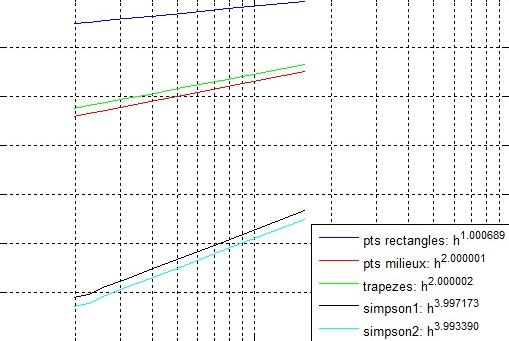
\includegraphics[scale=0.7]{./img/methods-order.jpeg}
    % methods-order.jpeg: 675x505 pixel, 96dpi, 17.86x13.36 cm, bb=0 0 506 379
    \caption{Les ordres des méthodes testées}
    \label{fig:order}
\end{figure}

\vspace*{2cm}

\begin{figure}[h!]
    \centering
    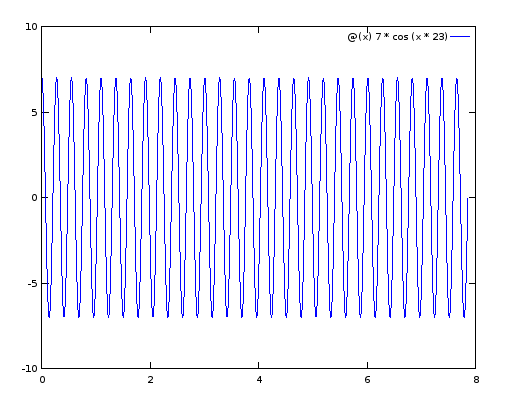
\includegraphics[scale=0.7]{./img/oscillant.png}
    % oscillant.png: 515x393 pixel, 96dpi, 13.62x10.40 cm, bb=0 0 386 295
    \caption{f(x) = 7cos(23x)}
    \label{fig:osc}
\end{figure}

\begin{figure}[h!]
    \centering
    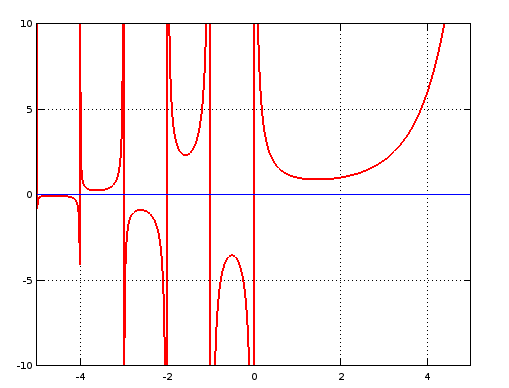
\includegraphics[scale=0.7]{./img/gamma-negative.png}
    % gamma-negative.png: 509x388 pixel, 96dpi, 13.47x10.26 cm, bb=0 0 382 291
    \caption{Le graphe de $\Gamma$ sur $[-5, 5]$}
    \label{fig:gamma}
\end{figure}

\begin{figure}[h!]
    \centering
    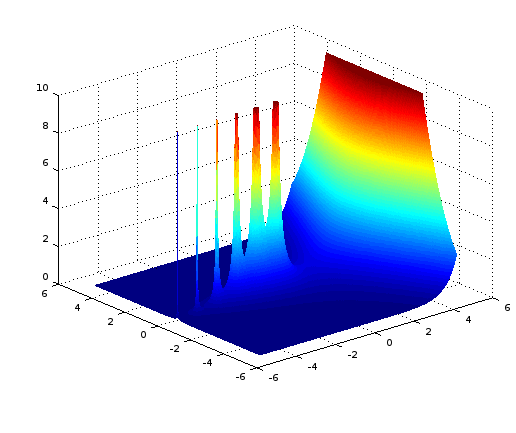
\includegraphics[scale=0.8]{./img/gamma-complex.png}
    % gamma-complex.png: 516x433 pixel, 96dpi, 13.65x11.46 cm, bb=0 0 387 325
    \caption{Le graphe de $\Gamma$ dans le plan complex}
    \label{fig:gcomplex}
\end{figure}

\end{document}
